\documentclass[12pt]{article}

\title{Fake News}
\author{Carmen Thom}
\date{04.03.2024}

\usepackage[margin=1in]{geometry}
\usepackage{floatrow} 
\usepackage{times}
\usepackage[table,xcdraw]{xcolor}
\usepackage{graphicx}
\graphicspath{ {./img/} }
\usepackage{caption}


\begin{document}
\maketitle


In a divisive world, 

Fake news semantics

For this project, the dataset used was WELFake dataset \textbf{9395133}. To diversify the sources, the original authors compiled sources from Kaggle, McIntire, Reuters, BuzzFeed Political. The dataset contains 72,134 news articles, 35,028 with label 1 for real, and 37,106 with label 0 for fake. The class proportions don't seem to have a statistically significant skew, meaning that the data appears well balanced. For fine tuning on this dataset, I went with 0.7 partitioned for training, with the .3 remaining being split between validation and testing. 

BERT models, as they use transformer architecture, excel at transfer learning. Thus, fine-tuning a pretrained BERT model was the best way to develop the classifier. For the pretrained model, I used Google's \verb|bert_uncased_L-4_H-512_A-8| model. This is significantly computationally easier to pretrain than the most used \verb|bert-base-uncased| model as the hidden size is reduced by a third, as well as fewer layers and attention heads. This change also reduced the odds of the fine-tuned binary classification model being over-fit. 

For fine-tuning, I used the transformers \verb|BertForSequenceClassification| built on PyTorch's neural network modules. A batch size of 64 was used to have less computational processes, although a lower batch size may have been ideal to help model generalization, and would keep keeps less data in local memory which is useful. I ran the model with 5 epochs. 3 may have been sufficient as the dataset is middle-sized, but checkpointing on training epochs was not implemented in the first run through so stopping when the model began to have marginal decreases in loss was not an option. \textbf{devlin2019bert} Checkpointing has now been implemented, but on a 8 core system, fine-tuning took approximately 4 hours. This could be greatly improved with access to a GPU, and with access to a Google Cloud TPU training should run well under an hour. For loss criterion, many of the academic and industrial papers fine-tuning BERT for binary sequence classification use a cross-entropy loss function which was also the criterion I chose. 

Throughout the training, accuracy increased 

Running the final evaluation script,

\textbf{Performance Metrics and Confusion Matrix}

\begin{minipage}{\textwidth}

\begin{minipage}[t]{.45\textwidth}
\centering
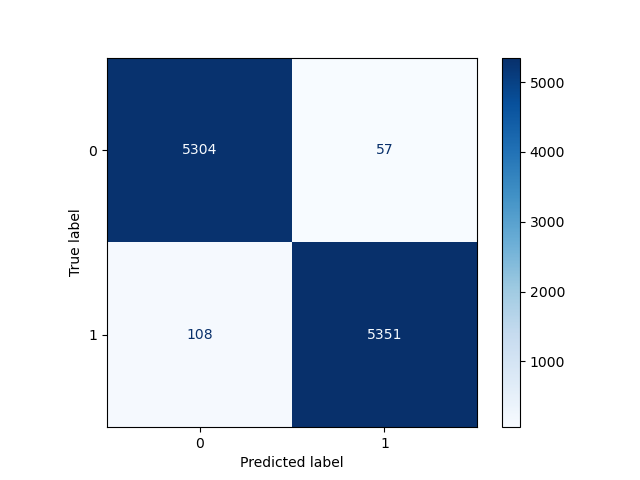
\includegraphics[width=0.7\textwidth]{confusion}
\captionof{figure}{Figure caption}% \caption{Figure caption}
\end{minipage}
\begin{minipage}[t]{.45\textwidth}
\resizebox{\textwidth}{!}{
\begin{tabular}{|
>{\columncolor[HTML]{F5F9FE}}l |l|l|l|l|}
\hline
\cellcolor[HTML]{08306B} & \multicolumn{1}{c|}{\cellcolor[HTML]{F5F9FE}Recall} & \multicolumn{1}{c|}{\cellcolor[HTML]{F5F9FE}Precision} & \multicolumn{1}{c|}{\cellcolor[HTML]{F5F9FE}F1-Score} & \multicolumn{1}{c|}{\cellcolor[HTML]{F5F9FE}Support} \\ \hline
0                        & 0.98                                                & 0.99                                                   & 0.98                                                  & 5361                                                 \\ \hline
1                        & 0.99                                                & 0.98                                                   & 0.98                                                  & 5459                                                 \\ \hline
Accuracy                 &                                                     &                                                        & 0.98                                                  & 10820                                                \\ \hline
Macro Average            & 0.98                                                & 0.98                                                   & 0.98                                                  & 10820                                                \\ \hline
Weighted Average         & 0.98                                                & 0.98                                                   & 0.98                                                  & 10820                                                \\ \hline
\end{tabular}
}
\end{minipage}
\end{minipage}
\\~\\


\textbf{Analysis:} The performance metrics and the confusion matrix provide a comprehensive overview of the model's accuracy and classification prowess.

looking at the sentences that underperformed

insights

conclusion
\end{document}